\newcommand{\adag}[1]{\hat{a}_{#1}^\dagger}
\newcommand{\aop}[1]{\hat{a}_{#1\vphantom{\dagger}}}
\chapter{Theory: \\ Background}
This chapter will cover the elementary concepts required to describe an membrane based optomechanical system in a quantum regime. We will first recall basics on optical field quantization as well describing coherent and squeezed light field, to then turn to the more specific frequency dependent squeezed light field. Secondly, we will cover the mathematical description of a mechanical resonator interacting with a generic coherent optical field, highlighting the differences with the seminal optomechanical system of a mirror on a spring. Finally, we will derive the equations of motions of a membrane based optomechanical system with frequency dependent squeezed optical fields. 
\minitoc
\newpage
\section{Quantum Optics Concepts}
\subsection{Quantum Description of Light}
We introduce briefly field quantization concepts needed to describe quasimonochromatic field propagation and measurements.

\subsection*{Quantised Electromagnetic Field}
% \the\textwidth

We consider the quantised electromagnetic field in volume $V$. The electric field operator can be expressed in the Heisenberg picture as:
\begin{equation}
\hat{\mathbf{E}}(\mathbf{r}, t) = i \sum_{ \ell} \mathcal{E}_l \left[\hat{a}_{\ell}^{\vphantom{dagger}}\mathbf{f}_{\ell}^{\vphantom{*}}(\mathbf{r})e^{-i\omega_{\ell}t} - \hat{a}_{\ell}^\dagger \mathbf{f}_{\ell}^*(\mathbf{r}) e^{i\omega_{\ell}t}\right]
\end{equation}
where $\mathcal{E}_l = \sqrt{\frac{\hbar \omega_l}{2 \varepsilon_0 V}}$ is the field per photon in mode $\ell$ with $\hbar$ the reduced Planck constant, $\omega_\ell$ the angular frequency of mode $\ell$ and $\varepsilon_0$ the vacuum permittivity, $\mathbf{f}_{\ell}(\mathbf{r})$ are spatial mode functions satisfying orthonormality, and ($\hat{a}_{\ell}^{\vphantom{\dagger}}$, $\hat{a}_{\ell}^{\dagger}$) are the time dependent annihilation and creation operators associated with each mode $\ell$ satisfying the canonical commutation relations
\[
[\hat{a}_{\ell}^{\vphantom{\dagger}}, \hat{a}_{\ell'}^\dagger] = \delta_{\ell \ell'} , \quad
[\hat{a}_{\ell}^{\vphantom{\dagger}}, \hat{a}_{\ell'}^{\vphantom{\dagger}} ] = 0, \quad [\hat{a}_{\ell}^\dagger , \hat{a}_{\ell'}^\dagger ] = 0  
\]
\subsection*{Fock basis}
In this description of the optical field, each mode $\ell$ is modeled as a quantum harmonic oscillator with a discrete set of energy eigenstates known as \textit{Fock states} or number states, denoted $\ket{n_\ell}$. These states form an orthonormal basis and satisfy $\hat{n}_{\ell} \ket{n_\ell} = n_\ell \ket{n_\ell}$, where $\hat{n}_{\ell}$ is the number operator defined by
\[
\hat{n}_{\ell} = \hat{a}_{\ell}^\dagger \hat{a}^{\vphantom{\dagger}}_{\ell}.
\]
The action of the creation and annihilation operators on these states is given by
\[
\hat{a}^{\vphantom{\dagger}}_{\ell} \ket{n_\ell} = \sqrt{n_\ell} \ket{n_\ell - 1}, \quad
\hat{a}_{\ell}^\dagger \ket{n_\ell} = \sqrt{n_\ell + 1} \ket{n_\ell + 1}.
\]
They allow transitions between Fock states by lowering or raising the photon number in mode $\ell$ by one unit. The vacuum state $\ket{0_\ell}$ is annihilated by $\hat{a}^{\vphantom{\dagger}}_{\ell}$, satisfying $\hat{a}^{\vphantom{\dagger}}_{\ell} \ket{0_\ell} = 0$. Thus, the Hamiltonian for the electromagnetic field becomes a sum of harmonic oscillator energies:
\begin{equation}
\hat{H} = \sum_\ell \hbar \omega_{\ell} \, \hat{a}_{\ell}^\dagger \hat{a}^{\vphantom{\dagger}}_{\ell} 
\end{equation}
where we ignore the constant zero-point energy term $\frac{1}{2} \hbar \omega_{\ell}$ for simplicity.

\subsection*{Quadrature Operators}

To describe the phase space properties of a field mode, we define the Hermitian quadrature operators $\hat{a}_{1}$ and $\hat{a}_{2}$ as
\begin{equation}
  \begin{split}
    \hat{a}_{1} &= \hat{a}^\dagger + \hat{a}^{\vphantom{\dagger}}   \\
    \hat{a}_{2} &= i(\hat{a}^{\dagger} - \hat{a})
  \end{split}
\end{equation}
More generally we can define arbitrary quadrature operators as 
\begin{align}
  \hat{a}_{\phi} &=\hat{a}  e^{-i\phi}+ \hat{a}^{\dagger} e^{i\phi} \notag \\ 
  & =  \hat{a}_{1} \cos \phi + \hat{a}_{2} \sin \phi 
\end{align}
where we notice that $\hat{a}_{1} = \hat{a}_{\phi=0\vphantom{\pi/2}}$ and $\hat{a}_{1} = \hat{a}_{\phi=\pi/2}$. These are Hermitian operators corresponding to measurable observables and satisfy the commutation relation
\begin{equation}
[\hat{a}_{\phi \vphantom{\pi/2}}, \hat{a}_{\phi+\pi/2}] = 2i
\end{equation}

\subsection*{Uncertainty Principle and Quantum Noise}

For two generic Hermitian operators $\hat{A}$ and $\hat{B}$, the Heisenberg uncertainty principle reads as 
\begin{equation}
  \Delta \hat{A}\Delta \hat{B} \geq \frac{1}{2} |[\hat{A}, \hat{B}]|
\end{equation}
where we define $\Delta \hat{A}=\sqrt{|\langle \hat{A}^2\rangle - \langle \hat{A} \rangle^2|}$. This defines the minimum amount of quantum noise (vacuum fluctuations) in the electromagnetic field.
Applying this equation to the quadratures defined above we get 
\begin{equation}
   \begin{split}
    \Delta \hat{a}_{1} \Delta \hat{a}_{2} &\geq 1 \\
    \Delta \hat{a}_{\phi \vphantom{\pi/2}} \Delta \hat{a}_{\phi +\pi/2} &\geq 1
   \end{split}
\end{equation}

\begin{figure}
\centering
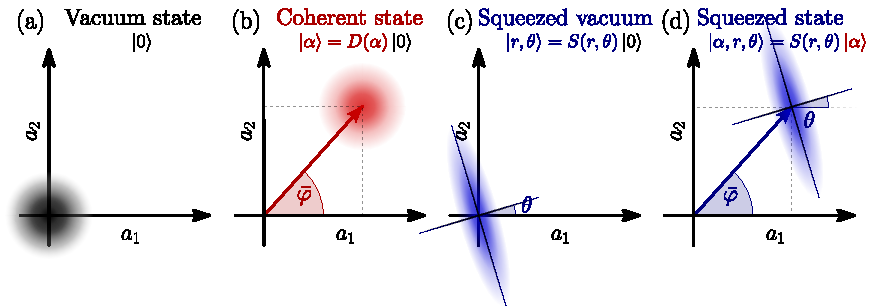
\includegraphics[width=\textwidth]{./chap2/fig/quantum_states.pdf}
\caption{Phase-space representations of quantum states and transformations.
(a) Wigner function of the vacuum state: a circular Gaussian centered at the origin, representing equal quantum fluctuations in both quadratures $a_1$ and $a_2$.
(b) Wigner function of a coherent state: a displaced circular Gaussian, showing a shift in phase space along an angle $\varphi$ with unchanged, isotropic noise.
(c) Wigner function of a squeezed vacuum state: an elliptical Gaussian centered at the origin, with reduced noise along a rotated quadrature $X_\theta$ and increased noise in the orthogonal direction.
(d) Wigner function of a displaced squeezed state: an ellipse shifted away from the origin, combining anisotropic fluctuations and a nonzero mean amplitude. The displacement angle $\varphi$ and squeezing angle $\theta$ are independent.} 
\end{figure}

\begin{figure}
\centering
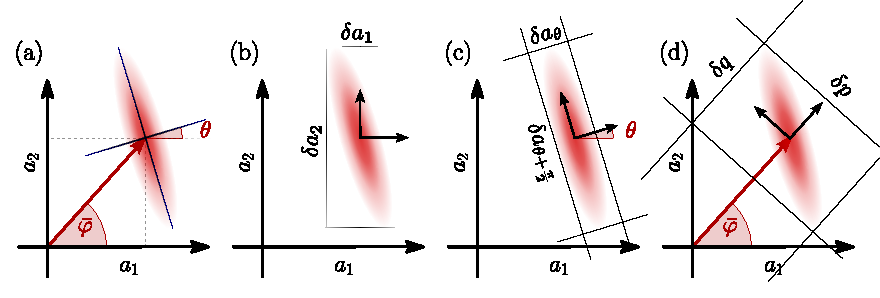
\includegraphics[width=\textwidth]{./chap2/fig/quantum_quadraturesBis.pdf}
\caption{Phase-space representations of quantum states and transformations.
(a) Wigner function of the vacuum state: a circular Gaussian centered at the origin, representing equal quantum fluctuations in both quadratures $X_1$ and $X_2$.
(b) Wigner function of a coherent state: a displaced circular Gaussian, showing a shift in phase space along an angle $\varphi$ with unchanged, isotropic noise.
(c) Wigner function of a squeezed vacuum state: an elliptical Gaussian centered at the origin, with reduced noise along a rotated quadrature $X_\theta$ and increased noise in the orthogonal direction.
(d) Wigner function of a displaced squeezed state: an ellipse shifted away from the origin, combining anisotropic fluctuations and a nonzero mean amplitude. The displacement angle $\varphi$ and squeezing angle $\theta$ are independent.} 
\end{figure}


We now turn to standard optical quantum states, in particular gaussian states i.e.\ full positive in Wigner function representations such as coherent and squeezed states, that we will denote in braket notation as $|\alpha\rangle$ and $|\alpha,r, \theta\rangle $.

\subsection*{Coherent States}
The coherent state $|\alpha\rangle$ is an eigenstate of the annihilation operator:
\begin{equation}
\hat{a}|\alpha\rangle = \alpha|\alpha\rangle
\end{equation}
where $\alpha = \alpha_0\, e^{i\bar{\varphi}}$ is a complex number representing the coherent amplitude. In this notation, $\alpha_0$ is itself a complex number whose fluctuations in both real and imaginary parts account for quantum fluctuations, and where the fixed angle $\bar{\varphi}$ i.e. the mean angle of the distribution is used to describe the relative phase to a reference (e.g. a local oscillator). Coherent states can be expressed in the Fock basis as: 
\begin{equation}
|\alpha\rangle = e^{-|\alpha|^2/2} \sum_{n=0}^{\infty} \frac{\alpha^n}{\sqrt{n!}} |n\rangle
\end{equation}
and are generated by the action of the displacement operator $\hat{D}(\alpha)$ on the vacuum state $|0\rangle$:
\begin{equation}
|\alpha\rangle = \hat{D}|0\rangle, \quad \hat{D}(\alpha) = \exp(\alpha \hat{a}^\dagger - \alpha^* \hat{a})
\end{equation}
For a coherent state $|\alpha\rangle$, the expectation values and variances of the quadrature operators are:
\begin{equation}
\begin{aligned}
  \langle \hat{a}_\phi \rangle &= 2\,\mathrm{Re}(\alpha e^{-i\phi}) \\
  \Delta \hat{a}_\phi^2 &= 1
\end{aligned}
\end{equation}
\begin{equation}
\begin{aligned}
  \langle a_{\phi \vphantom{\pi/2}} \rangle &= 2\,\mathrm{Re}(\alpha_0 e^{i(\bar{\varphi}-\phi)}) \\
  \langle a_{\phi+\pi/2} \rangle &= 2\,\mathrm{Im}(\alpha_0 e^{i(\bar{\varphi}-\phi)}) \\
    \Delta a_{\phi \vphantom{+\pi/2}}^2 &= 1, \quad \Delta , a_{\phi+\pi/2}^2 = 1
\end{aligned}
\end{equation}

That is, the mean value of any quadrature is set by the coherent amplitude, while the variance is unity (in these units) for all quadratures. The mean and variance of the photon number in a coherent state are given by: 
\begin{equation}
  \begin{split}
    \langle \hat{N} \rangle &= |\alpha_0|^2 \\
    \Delta N ^2 &= |\alpha_0|^2
  \end{split}
\end{equation}
Coherent states are often referred to as "classical" states of light because they exhibit Poissonian photon statistics and minimal uncertainty in phase space, making them the closest quantum analog to classical electromagnetic waves. \\

Conveniently, we define the amplitude and phase quadrature operators as:
\begin{equation}
  \begin{split}
    \hat{p} &= \hat{a}_{\phi=\bar{\varphi}\vphantom{\pi/2}}  \\
    \hat{q} &= \hat{a}_{\phi=\bar{\varphi}+\pi/2}
  \end{split}
\end{equation}
with expectation values and variances:  
\begin{equation}
\begin{aligned}
  \langle \hat{p} \rangle &= 2\,\mathrm{Re}(\alpha_0 ) \\
  \langle \hat{q} \rangle &= 2\,\mathrm{Im}(\alpha_0) \\
  \Delta \hat{p}^2 &= 1, \quad \Delta \hat{q}^2 = 1
\end{aligned}
\end{equation}

\subsection*{Squeezed States}

Squeezed states $|\alpha, r, \theta\rangle $ are quantum gaussian states of light in which the noise (variance) of one quadrature is reduced below the vacuum level, at the expense of increased noise in the conjugate quadrature. The single-mode squeezed vacuum state is defined as
\begin{align}
|0, r, \theta \rangle = \hat{S}(r, \theta) |0\rangle , \quad \hat{S}(\theta) = \exp\left[\frac{r}{2}(e^{-i\theta} \hat{a}^2 - e^{-i\theta} \hat{a}^{\dagger 2})\right]
\end{align}
where $r$ is the squeezing parameter (strength) and $\theta$ is the squeezing angle. The most general Gaussian state is the displaced squeezed state, obtained by applying both the squeezing operator $\hat{S}(r, \theta)$ and the displacement operator $\hat{D}(\alpha)$ to the vacuum:
\begin{equation}
|\alpha, r, \theta\rangle = \hat{D}(\alpha)\hat{S}(r, \theta)|0\rangle
\end{equation}
where $\hat{D}(\alpha)$ displaces the state in phase space by the complex amplitude $\alpha$.\\


\color{red}
WATCH OUT THIS IS NOT TRUE (ONLY FOR VACUUM) --> TO REWRITE 
\color{black}
For $\theta = \bar{\varphi}$ (amplitude quadrature squeezing), the quadrature variances become
\begin{equation}
\Delta \hat{p} = \frac{e^{-r}}{\sqrt{2}}, \qquad \Delta \hat{q} = \frac{e^{r}}{\sqrt{2}}
\end{equation}
where their respective product saturating the Heisenberg uncertainty relation: it is a minimum uncertainty state.\\ 

\noindent \textbf{Note:}  The displacement and squeezing operators do not commute, i.e., $\hat{D}(\alpha)\hat{S}(\xi) \neq \hat{S}(\xi)\hat{D}(\alpha)$. However, both orderings correspond to experimentally valid procedures: one can either squeeze the vacuum and then displace (e.g. by mixing with a coherent state ona beamsplitter), or squeeze a coherent state straight away (e.g. by seeding an optical parametric amplifier). The resulting state is always a displaced squeezed state, but the relative phase between displacement and squeezing may differ. \\

The mean photon number in the squeezed state is: 
\begin{equation}
\langle \hat{N} \rangle = \langle \alpha, r, \theta | \hat{a}^\dagger \hat{a} | \alpha, r, \theta \rangle = |\alpha_0|^2 + \sinh^2 r 
\end{equation}
This shows that the squeezing operation increases the mean photon number of the coherent state by adding photons. Physically, this reflects the fact that generating squeezed light requires injecting energy into the system, so the squeezed vacuum contains correlated field excitations (photons) in even numbers. This is further illustrated by the two-mode squeezing operator, which describes the simultaneous creation or annihilation of photon pairs in two modes (such as upper and lower sidebands or two distinct modes):
\begin{equation}
\hat{S}_2(\xi) = \exp\left[ \xi^* \hat{a}_{+} \hat{a}_{-} - \xi \hat{a}_{+}^\dagger \hat{a}_{-}^\dagger \right], \quad \xi = r e^{i\phi}
\end{equation}
The expectation values of the annihilation operators $\hat{a}_{+}$ and $\hat{a}_{-}$ in a two-mode squeezed vacuum state $|\xi\rangle = \hat{S}_2(\xi)|0\rangle$ are both zero:
\begin{equation}
\langle \xi | \hat{a}_{+} | \xi \rangle = 0, \qquad \langle \xi | \hat{a}_{-} | \xi \rangle = 0
\end{equation}
This reflects that the two-mode squeezed vacuum has zero mean field in both modes. However, the expectation value of the product $\hat{a}_{+} \hat{a}_{-}$ is nonzero:
\begin{equation}
\langle \xi | \hat{a}_{+} \hat{a}_{-} | \xi \rangle = -e^{i\phi} \sinh r \cosh r
\end{equation}
where $\xi = r e^{i\phi}$ is the squeezing parameter. This nonzero correlation is a hallmark of two-mode squeezing and underlies quantum entanglement between the modes.
This form describes two-mode squeezing, where photon pairs are created or annihilated simultaneously in the $+$ and $-$ modes. For $\phi = 0$, the squeezing is along the amplitude quadrature; for $\phi = \pi/2$, along the phase quadrature. This operator is central to the description of squeezed vacuum states generated by parametric down-conversion and is widely used in quantum optics and optomechanics.

In quantum optics, a two-mode squeezed vacuum state arises from the parametric down-conversion of a pump field at frequency \(2\omega\), producing pairs of photons at symmetric sideband frequencies \(\omega \pm \Omega\). The resulting state is a pure entangled superposition of twin Fock states, of the form
\[
|\psi\rangle = \sum_{n=0}^{\infty} c_n\, |n\rangle_+ \otimes |n\rangle_- , \quad \text{with} \quad c_n \propto \tanh^n r,
\]
where \(r\) is the squeezing parameter. Importantly, when one sideband is traced out, the reduced state of the remaining mode becomes a thermal state with a Bose-Einstein photon number distribution
\[
P_n = \frac{\bar{n}^n}{(\bar{n} + 1)^{n+1}}, \quad \text{with} \quad \bar{n} = \sinh^2 r.
\]
This thermal character is not due to any external bath but results from quantum entanglement and the loss of information associated with ignoring one mode of the pair. The corresponding Wigner function is isotropic and broader than that of vacuum, with quadrature variances
\[
\langle \hat{X}^2 \rangle = \langle \hat{Y}^2 \rangle = \bar{n} + \frac{1}{2},
\]
reflecting excess fluctuations in all directions of phase space. In contrast, a single-mode squeezed vacuum involves an even-parity superposition,
\[
|\xi\rangle = \sum_{n=0}^{\infty} d_{2n}\, |2n\rangle,
\]
resulting from the same parametric process but in a degenerate configuration where photons are created in indistinguishable pairs. While single-mode squeezing yields quadrature-dependent noise (an elliptical Wigner function), its photon statistics also reveal the underlying pairwise structure of the interaction. Crucially, both processes involve the coherent transformation of vacuum fluctuations rather than thermal excitations. At optical frequencies (\(\omega \sim 300\,\mathrm{THz}\)) and room temperature (\(T = 300\,\mathrm{K}\)), the thermal occupation
\[
\bar{n}_{\text{th}} = \frac{1}{e^{\hbar \omega / k_B T} - 1} \sim 10^{-20}
\]
is entirely negligible. This stark contrast between thermal and quantum (entanglement-induced) noise is essential to interpreting squeezed state measurements and correctly identifying the quantum origin of excess fluctuations observed in individual modes.



\subsection*{Quasi monochromatic fields } 
In realistic optical systems such as lasers, the electromagnetic field is rarely perfectly monochromatic. Instead, it exhibits a finite spectral linewidth due to stimulated emission, phase noise, or intentional modulation. These effects cause the amplitude and phase of the optical field to evolve slowly compared to the optical frequency $\omega_\ell$. \\

As a result, the complex amplitude associated with each mode, typically captured by the Heisenberg-picture annihilation operator $\hat{a}_\ell$, acquires an explicit time dependence beyond the standard fast-oscillating term $e^{-i\omega_\ell t}$. This slow temporal variation reflects the underlying physics: for instance, amplitude or phase modulation, feedback-induced dynamics, or noise processes can all modulate the quantum state in time. Consequently, in the quasi-monochromatic regime, one often separates the field into a rapidly oscillating carrier and a slowly varying envelope encoded in $\hat{a}_\ell(t)$, allowing a spectrally resolved yet temporally adaptive description of the field. \\

\subsection*{Linearization of the optical field: mean field and fluctuations}

We often consider a single spatial mode of the electromagnetic field with optical frequency \(\omega_0\), and assume the presence of a strong coherent field. In this regime, the annihilation operator is decomposed as \(\hat{a}(t) = \alpha(t) + \delta\hat{a}(t)\), where \(\alpha(t)=\langle \hat{a}(t)\rangle\) is now the classical complex amplitude and \(\delta\hat{a}(t)\) represents quantum fluctuations such that \(\langle \delta \hat{a}(t)\rangle=0\). \\ 

Linearizing the electric field operator then yields:
\begin{equation}
\begin{aligned}
\hat{\mathbf{E}}(\mathbf{r}, t) 
&= i \, \mathcal{E} \left[ \alpha(t)\, \mathbf{f}(\mathbf{r})\, e^{-i \omega_0 t} 
- \alpha^*(t)\, \mathbf{f}^*(\mathbf{r})\, e^{i \omega_0 t} \right] \\
&\quad + i \, \mathcal{E} \left[ \delta \hat{a}(t)\, \mathbf{f}(\mathbf{r})\, e^{-i \omega_0 t}
- \delta \hat{a}^\dagger(t)\, \mathbf{f}^*(\mathbf{r})\, e^{i \omega_0 t} \right]
\end{aligned}
\end{equation} \\

The first line represents the field classical component, involving the coherent amplitude $\alpha(t)$, while the second shows the quantum fluctuation term $\delta\hat{a}(t)$. This linearization simplifies the analysis of the field, allowing us to treat the coherent part as a classical field and the fluctuations as a quantum harmonic oscillator. The field Hamiltonian then reduces to a single-mode harmonic oscillator form:
\begin{equation}
\hat{H} = \hbar \omega_0 \left( \delta \hat{a}^\dagger \delta \hat{a} + \frac{1}{2} \right),
\end{equation}
where $\delta \hat{a}$ is the annihilation operator for the fluctuations. The coherent part contributes a constant energy offset, while the fluctuations behave as a quantum harmonic oscillator with frequency $\omega_0$. This Hamiltonian now features an explicit time dependence through the coherent amplitude $\bar{\alpha}(t)$, which can vary slowly compared to the optical frequency.
Importantly, the fluctuation operators retain the canonical bosonic commutation relations:
\[
[\delta \hat{a}(t), \delta \hat{a}^\dagger(t)] = 1, \qquad
[\delta \hat{a}(t), \delta \hat{a}(t)] = 0, \qquad
[\delta \hat{a}^\dagger(t), \delta \hat{a}^\dagger(t)] = 0.
\]
These ensure that the quantized nature of the field is preserved under linearization, with $\delta \hat{a}(t)$ and $\delta \hat{a}^\dagger(t)$ obeying the same algebra as the original field operators. The number operator can then be written as the sum of a constant (mean) part and a fluctuation part:
\begin{equation}
\hat{n}(t) = \hat{a}^\dagger(t)\hat{a}(t) = |\alpha(t)|^2 + \alpha^*(t)\delta\hat{a}(t) + \alpha(t)\delta\hat{a}^\dagger(t) + \delta\hat{a}^\dagger(t)\delta\hat{a}(t)
\end{equation}
where the constant (mean) part is simply
\begin{equation}
\bar{n}(t) = |\alpha(t)|^2
\end{equation}
and the remaining terms describe the quantum fluctuations around this mean. \\

\noindent \textbf{Remarks:} 
\begin{itemize}
  \item The linearization procedure is valid when the coherent amplitude $\bar{\alpha}(t)$ is much larger than the quantum fluctuations, i.e., $|\bar{\alpha}(t)| \gg \langle \delta\hat{a}^\dagger \delta\hat{a} \rangle^{1/2}$.
  \item This approach is widely used in quantum optics and optomechanics to simplify the analysis of systems driven by strong gaussian fields, such as coherent or squeezed lasers.
  \item The separation into mean field and fluctuations allows us to treat the quantum noise properties independently from the classical dynamics.
  \item The quantum fluctuation operators $\delta\hat{a}(t)$ and their spectra will eventually describe vacuum or squeezed noise, and their statistics determine the ultimate sensitivity limits in measurement schemes.
  \item Linearization is the starting point for deriving quantum Langevin equations and for analyzing noise spectra in optomechanical systems.
\end{itemize}



\vspace{1em}
This concludes our introduction to the quantum description of light, setting the stage for modelling interactions between quantum optical fields and mechanical resonators.

\subsection{Classical Sidebands}

We consider a single optical mode with a strong coherent drive, and we set $\bar{\varphi}=0$ for notational simplicity.

\subsubsection*{Amplitude Modulation (AM)}

Let the classical coherent amplitude be modulated in amplitude:
\begin{equation}
  \alpha(t) = \alpha_0(t) \left(1 + \epsilon_a \cos(\Omega t)\right)
\end{equation}
with $\epsilon_a \ll 1$, the field amplitude modulation depth. Substituting into the field expression and dropping the spatial mode functions for clarity:
\begin{align}
  E_{\text{cl}}^{\text{(AM)}}(t) =
  i \sqrt{\frac{\hbar \omega_0}{2 \varepsilon_0}}\,\alpha_0(t) \Big[
  &\underbrace{e^{-i\omega_0 t} - e^{i\omega_0 t}}_{\text{carrier}} \notag \\
  &+ \underbrace{\frac{\epsilon_a}{2} \left( e^{-i(\omega_0 - \Omega)t} - e^{i(\omega_0 - \Omega)t} \right)}_{\text{lower sideband } (\omega_0 - \Omega)} \notag \\
  &+ \underbrace{\frac{\epsilon_a}{2} \left( e^{-i(\omega_0 + \Omega)t} - e^{i(\omega_0 + \Omega)t} \right)}_{\text{upper sideband } (\omega_0 + \Omega)}
  \Big]
\end{align}

\subsubsection*{Phase Modulation (PM)}
Now consider phase modulation of the coherent amplitude:
\begin{align}
  \alpha(t) &= \alpha_0(t) e^{i \epsilon_\phi \cos(\Omega t)} \\ \notag
  &\approx \alpha_0 \left(1 + i \epsilon_\phi \cos(\Omega t)\right) \\
  & \approx \alpha_0 \left(1 + \frac{i \epsilon_\phi}{2} e^{i\Omega t} + \frac{i \epsilon_\phi}{2} e^{-i\Omega t} \right)\notag
\end{align}
with $\epsilon_\phi \ll 1$, the field phase modulation depth. Substituting into the field expression and dropping the spatial mode functions:
\begin{align}
  E_{\text{cl}}^{\text{(PM)}}(t) =
  i \sqrt{\frac{\hbar \omega_0}{2 \varepsilon_0}}\, \alpha_0(t) \Big[
  &\underbrace{e^{-i\omega_0 t} - e^{i\omega_0 t}}_{\text{carrier}} \notag \\
  &+ \underbrace{\frac{i \epsilon_\phi}{2} \left( e^{-i(\omega_0 - \Omega)t} + e^{i(\omega_0 - \Omega)t} \right)}_{\text{lower sideband } (\omega_0 - \Omega)} \notag \\
  &+ \underbrace{\frac{i \epsilon_\phi}{2} \left( e^{-i(\omega_0 + \Omega)t} + e^{i(\omega_0 + \Omega)t} \right)}_{\text{upper sideband } (\omega_0 + \Omega)}
  \Big]
\end{align}
\subsection*{Interpretation}
In both cases, the field contains a carrier at frequency $\omega$ and two sidebands at $\omega \pm \Omega$. Amplitude modulation results in sidebands that are in phase with the carrier, while phase modulation produces sidebands with a $\pm \pi/2$ phase shift relative to the carrier.

\subsection{Quantum Sidebands - Two Photon Model }
We begin by recalling the quantized electric field operator for a single spatial mode with carrier frequency $\omega_0$ and mode function $\mathbf{f}(\mathbf{r})$ (as in Eq.~II.1):
\begin{equation}
\hat{\mathbf{E}}(\mathbf{r}, t) = i \mathcal{E} \left[ \hat{a}(t)\, \mathbf{f}(\mathbf{r})\, e^{-i \omega_0 t} - \hat{a}^\dagger(t)\, \mathbf{f}^*(\mathbf{r})\, e^{i \omega_0 t} \right]
\end{equation}
where $\hat{a}(t)$ is the slowly varying annihilation operator in the rotating frame.
To analyze the field in the sideband representation, we express the annihilation operator in terms of its Fourier components over positive frequencies:
\begin{equation}
\hat{a}(t) = \int_0^\infty \frac{d\omega}{2\pi} \, \hat{a}(\omega) e^{-i\omega t} 
\end{equation}
We introduce a central carrier frequency \( \omega_0 \) and define sideband frequencies via \( \Omega = \omega_0 - \omega \). Furthermore, we assume that the field is band-limited to a finite bandwidth \( B \) around the carrier frequency, which reduces the shifted range of integration to :
\[
\omega \in [0, \infty[ \quad \Rightarrow \quad \Omega \in [-\omega_0, \infty[ \quad \Rightarrow \quad \Omega \in [-B, B[
\]
so that the expression reduces to 
\begin{equation}
\hat{a}(t) 
= e^{-i \omega_0 t }\int_{-B}^{B} \frac{d\Omega}{2\pi} \, \hat{a}_+(\Omega)  e^{-i(\Omega)t}
\end{equation}
where we defined the sideband annihilation operators:
\begin{equation}
\hat{a}_+(\Omega) := \hat{a}(\omega_0 + \Omega), \quad
\hat{a}_-(\Omega) := \hat{a}(\omega_0 - \Omega)
\end{equation}
The above field expression is then succintly written as: 
\begin{equation}
  \hat{a}(t) = e^{-i \omega_0 t }\int_{0}^{B} \frac{d\Omega}{2\pi} \left[ \hat{a}_+(\Omega) e^{-i\Omega t} + \hat{a}_-(\Omega) e^{i\Omega t} \right]
\end{equation}


\section{Optical Cavities: Basics}
\subsection{Cavity types and Resonance Conditions}
\subsection{Spatial and Longitudinal Modes}
\subsection{Quantum Langevin Equations}

We consider a bosonic mode described by the annihilation operator \(\hat{a}(t)\), interacting with several independent Markovian reservoirs. The system is governed by a Hamiltonian \(\hat{H}_\mathrm{sys}\), and each reservoir introduces dissipation characterized by a decay rate \(\kappa_i\). In the Heisenberg picture, the dynamics of \(\hat{a}(t)\) is given by the quantum Langevin equation:
%
\begin{equation}
\frac{d}{dt} \hat{a}(t) = -i [\hat{a}, \hat{H}_\mathrm{sys}] - \frac{\kappa}{2} \hat{a}(t) + \sum_i \sqrt{\kappa_i} \, \hat{a}_{\mathrm{in},i}(t),
\label{eq:qle}
\end{equation}
where:
\begin{itemize}
  \item \(\kappa = \sum_i \kappa_i\) is the total decay rate,
  \item \(\hat{a}_{\mathrm{in},i}(t)\) are the input noise operators associated with each reservoir.
\end{itemize}
The input fields \(\hat{a}_{\mathrm{in},i}(t)\) model quantum fluctuations entering the system from each bath. For uncorrelated reservoirs in the vacuum state, these noise operators satisfy the following correlation and commutation relations:
%
\begin{align}
\left[ \hat{a}_{\mathrm{in},i}(t), \hat{a}^\dagger_{\mathrm{in},j}(t') \right] &= \delta_{ij} \, \delta(t - t'), \\
\langle \hat{a}_{\mathrm{in},i}(t) \hat{a}^\dagger_{\mathrm{in},j}(t') \rangle &= \delta_{ij} \, \delta(t - t'), \\
\langle \hat{a}^\dagger_{\mathrm{in},i}(t) \hat{a}_{\mathrm{in},j}(t') \rangle &= 0.
\end{align}
Equation~\eqref{eq:qle} encapsulates the interplay between coherent evolution driven by the system Hamiltonian, dissipation into multiple channels, and quantum noise introduced by each reservoir. This structure is particularly relevant in cavity and circuit quantum electrodynamics, where a single bosonic mode (e.g., an optical or microwave cavity) is simultaneously coupled to several loss ports (e.g., transmission lines, internal losses, or detection chains).

\section{Squeezed Light Theory}
\subsection{Single-mode Squeezing}
\subsection{Noise Spectra }
\subsection{Frequency-dependent Squeezing and its use}

\section{Numerical Methods and Simulations}
